% REVISÃO DE LITERATURA--------------------------------------------------------

\chapter{REVISÃO DA LITERATURA}
\label{chap:fundamentacaoTeorica}
Neste capítulo será feita uma revisão da literatura necessária para o entendimento deste trabalho de conclusão de curso. 
Serão abordados os temas como: o processo de inicialização de um sistema embarcado, o que é um \bootloader\ e o papel do \linker\ na criação de um arquivo executável e no mapeamento da memória da aplicação.
Também será discutido sobre  a comunicação cliente-servidor, a pilha TCP/IP, a biblioteca LwIP e alguns protocolos implementados por ela, assim como a biblioteca Mbed TLS, alguns protocolos e algoritmos de segurança implementados por ela.
Será mostrado o que é um sistema de arquivo, o sistema de arquivos FAT e a biblioteca FatFs.
Com o conhecimento obtido sobre todos esses temas o leitor será capaz de compreender como será desenvolvido o método de atualização de \firmware\ OTA.


%\section{PLATAFORMA EMBARCADA — STM32F7 DISCOVERY}%materiais
%\section{SISTEMAS EMBARCADOS}
%\subsection{ARM M7 E SUA FAMÍLIA.}
%\section{FIRMWARE OVER THE AIR}
%O conceito de \textit{firmware over the air} (FOTA),  consiste em um mecanismo de atualização remoto de firmware, já é muito utilizado em firmware de smartfones por fornecer uma forma segura, eficiente e conveniente de atualização.geralmente utilizado em smartfones.  
\section{PROCESSO DE INICIALIZAÇÃO DO SISTEMA}

Segundo \citeonline{Qing2003}, um processador embarcado, após ser ligado, busca e executa o código de um endereço pré-definido e gravado permanentemente na memória. O código contido nessa localização da memória é chamado de \resetv. O \resetv\ é usualmente uma instrução de salto para outro espaço da memória em que o real código de inicialização se encontra. A razão deste salto para outra localidade da memória é para manter o \resetv\ pequeno. O \resetv\ pertence a uma pequena área da memória reservada pelo sistema por motivos especiais. O \resetv, assim como o código de inicialização do sistema, precisa estar armazenado permanentemente. Por causa deste problema, o código de inicialização, chamado de código \textit{bootstrap}, reside na memória somente de leitura (ROM), na flash ou em outra memória não volátil. O termo \textit{loader} se refere ao código que é responsável por executar o \textit{bootstrap}, fazer o possível \download\ de uma imagem de outro local e inicialização da aplicação final.

O conceito é melhor explicado por meio de um exemplo. Neste exemplo, iremos assumir que o \loader\ foi desenvolvido e programado na memória flash. Além disso, será assumido que a imagem alvo contém várias seções de programa. Cada seção tem um lugar designado no mapa de memória. O \resetv\ está contido em uma pequena ROM, que está mapeada na localização 0x0h do espaço de endereços. A ROM contém alguns valores iniciais essenciais requeridos pelo processador quando o sistema é reinicializado (\textit{reset}). Esses valores são o \resetv, o \textit{stack pointer} (ponteiro de pilha) inicial e o endereço da memória de acesso randômico (RAM) usável. 

No exemplo ilustrado na \autoref{fig:INICIALIZAÇÃO}, o \resetv\ é uma instrução de salto para o endereço de memória 0x00040h; o \resetv\ transfere o controle do programa para a instrução neste endereço. O código de inicialização do sistema contém, entre outras coisas o programa \loader\ da imagem destino e o vetor de exceção padrão do sistema (\textit{exception vector}). O vetor de exceção do sistema aponta para uma instrução que reside na memória flash.

A primeira parte do processo de \textit{bootstrap} do sistema é colocar o sistema em um estado conhecido. São colocados valores padrões apropriados nos registradores do processador. São colocados no \stackp\ os valores encontrados na ROM. O \loader\ desabilita as interrupções do sistema, pois o sistema ainda não está preparado para lidar com interrupções. O \loader\ também inicializa a memória RAM e possivelmente a \textit{cache} (memória transitória) do processador. Neste ponto, o \loader\ executa um diagnóstico de \textit{hardware} limitado nos dispositivos necessários para essas operações.

A execução do programa é mais rápida na RAM quando comparada ao mesmo código executado diretamente na memória flash. O \loader\ pode opcionalmente copiar o código da memória flash para a RAM. Por causa dessa capacidade, uma seção de programa pode tanto ter um endereço de carregamento, quanto um endereço de execução. O endereço de carregamento é onde a seção do programa reside, enquanto o endereço de execução é o endereço em que o \loader\ copia a seção do programa e a prepara para a execução.

\begin{figure}[H]
    \scriptsize
     \centering
     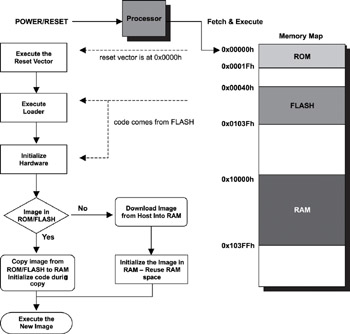
\includegraphics[scale=1]{dados/figuras/BootOriginal.png}
     \caption{Processo de inicialização de um sistema embarcado.\newline Fonte:\cite{Qing2003}}
     \label{fig:INICIALIZAÇÃO}
\end{figure}

Uma imagem executável possui seções de dados inicializados e não inicializados. Essas seções são ambas legíveis e graváveis. Essas seções precisam residir na RAM, assim sendo são copiadas da memória flash para a RAM como parte do sistema de inicialização. A seção de dados inicializados (chamadas pelo \linker\ de .data e .sdata) contém os valores iniciais para as variáveis globais e estáticas. O contéudo dessa seção, portanto, faz parte da imagem executável final e é transferido completamente pelo \loader. Por outro lado, o contéudo da seção de dados não inicializado (chamado pelo \linker\ de .bss e .sbss) é vazio. O \linker\ reserva espaço para essa seção no mapa de memória. As informações de alocação dessas seções, como o tamanho da seção e o endereço de execução da seção, são parte do cabeçalho da seção. É trabalho do \loader\ obter essas informações dos cabeçalhos de seção e alocar a mesma quantidade de memória na RAM durante o processo de carregamento. O \loader\ coloca essas seções na RAM de acordo com o endereço de execução das seções.

Uma imagem executável provavelmente possui constantes. Os dados das contantes são parte da seção chamada pelo \linker\ de .const, que é somente leitura. Sendo assim, é possível manter a seção .const na memória somente de leitura durante a execução do programa. Constantes de acesso frequente, como tabelas de \textit{lookup}, necessitam ser transferidas para a RAM para melhorar o desempenho do sistema.

O próximo passo no processo de inicialização do sistema é o \loader\ inicializar os dispositivos do sistema. Apenas os dispositivos necessários são inicializados nessa etapa. Em outras palavras, um dispositivo é inicializado na medida em que um subconjunto necessário dos recursos e recursos do dispositivo estejam ativados e operacionais. Geralmente, os dispositivos são parte da interface de entrada e saída do sistema, portanto, esses dispositivos são completamente iniciados quando existe a necessidade de se fazer \download\ de uma imagem de outro local.

Agora o \loader\ está pronto para transferir a imagem da aplicação para o sistema alvo. A imagem da aplicação pode conter um RTOS, um \textit{kernel}, e os demais códigos das aplicações que o desenvolvedor necessita.


%Conhecer o processo de inicialização dos sistemas embarcados, também chamado de \boot, é muito importante para nos dar noção sobre quando e como entrará em execução tanto a aplicação final, quanto o bootloader.
%Dependendo do fabricante do \textit{chip} o \boot pode ser diferente, porém geralmente ele segue a mesma linha de execução, podendo ou não ter interfaces físicas para mudar a origem do \boot. Algumas placas da ST \cite{ST2019}, contém um mecanismo chamado de \textit{physic remap}, para que o \boot ocorra a partir de outras memórias e não da Flash, que é a padrão \cite{Noviello2018}.

%Como dito por \citeonline{Beningo2015}, o fluxo padrão de \boot do sistema consiste em, após a tensão de referência de um microcontrolador se estabilizar, o processador procura pelo vetor de \textit{reset}, para a obter a localização da instrução de iniciação na Flash. O vetor de reset esta localizado em um endereço especial da memória FLASH, geralmente no início. Como pode ser visto na imagem \ref{MAP_PIC24F16KLXXX} que contém o mapa de memória do MCU (\textit{microcontroller unit}) PIC24F16KLXXX, o vetor de \textit{reset} se encontra no endereço 0x0002.

%\begin{figure}[H]
 %   \scriptsize
 %    \centering
     %\includegraphics[scale=1]{dados/figuras/%ResetVector.jpg}
     %\caption{Mapa de memória do MCU PIC24F16KLXXX.\newline Fonte: \cite{Beningo2015}}
     %\label{MAP_PIC24F16KLXXX}
%\end{figure}

%Então o endereço contido no vetor de \textit{reset} é carregado pelo microcontrolador, e a instrução contida neste endereço é carregada e executada pelo processador. Essa instrução ainda não é a \textit{main} que foi desenvolvida pelo projetista, ela é somente uma instrução de como o MCU irá iniciar. Esta instrução geralmente tem como função copiar o \textit{Vector Table} que esta na memória FLASH para a RAM, copiando e escrevendo em um endereço determinado pelo arquivo de \linker.

%As variáveis que são inicializadas durante o tempo de compilação que estão armazenadas na seção \textit{.data} do arquivo de \linker são então gravadas na memória RAM, e as variáveis não inicializadas explicitamente ou iniciadas com zero que estão na seção \textit{.bss} do arquivo de \linker, são guardadas na memória RAM. O MCU então copia funções que estão na FLASH para a RAM, essa etapa é opcional, o projetista tem que determinar se alguma função deve necessariamente ser executada a partir da memória RAM. 

%Todo esse processo é chamado de \textit{"C Copy Down"}, que faz a preparação do ambiente para iniciar uma aplicação, após essa etapa ser concluída o MCU pode então chamar a função \textit{main}, que é a \firmware principal do sistema desenvolvido pelo projetista. Toda a sequência padrão de \textit{boot} pode ser observada na \autoref{Seq_Boot}.

%\begin{figure}[H]
 %   \scriptsize
  %   \centering
   %  
\includegraphics[scale=1]{dados/figuras/ToDo.jpg}
    % \caption{Sequencia de Boot.}
     %\label{Seq_Boot}
%\end{figure}

%É possível alterar a função da tarefa contida no vetor de \textit{reset} no arquivo de \linker, fazendo com que o MCU passe pelo processo de \textit{C Copy Down}, preparando o sistema para outra função diferente da aplicação principal do sistema embarcado, como é utilizado na criação de um \bootloader para a atualização de \firmware.













\subsection{BOOTLOADER}

O \bootloader\ é um \textit{software} que tem como responsabilidade a atualização do \firmware\ do sistema, operação também conhecida como \textit{in-aplicattion programing} (IAP). Reside em uma área protegida da memória, geralmente colocado no início da flash ou na ROM, e é o primeiro \textit{software} a ser executado após o \textit{reset} ou iniciação do sistema.
É desenvolvido para receber comandos via periféricos de comunicação como: UART, I2C, SPI, CAN e Ethernet, e entender o mapa de memória do microcontrolador \cite{DavesDurlin2013}. A \autoref{Diag_Bootloader} mostra como geralmente fica alocado um \bootloader\ e o \firmware\ na memória.
% que são usados para trocar do firmware do MCU e recebimento do novo código de aplicação. Frequentemente é necessário um programa externo para dar esses comandos ao bootloader \cite{Noviello2018}.

\begin{figure}[H]
    \scriptsize
     \centering
     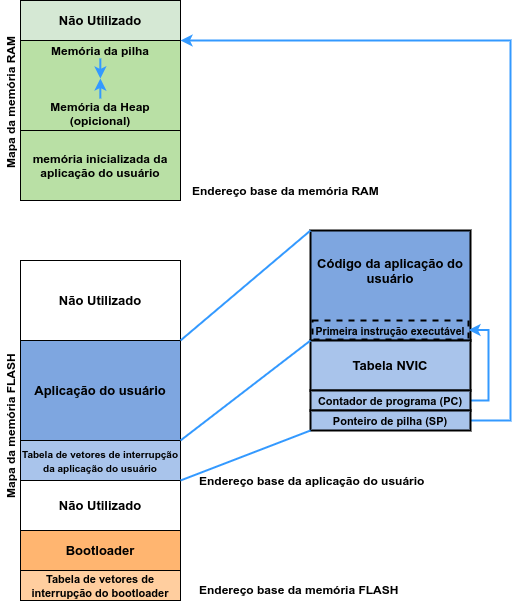
\includegraphics[scale=0.7]{dados/figuras/DiagBootloaderOriginal.png}
     \caption{Alocação do bootloader e firmware nas memórias flash e ram.\newline Fonte:\cite{DavesDurlin2013}}
     \label{Diag_Bootloader}
\end{figure}

Sua função se resume geralmente a: comunicar-se com outro servidor, ler os arquivos enviados pelo \textit{host}, atualizar o \firmware\ de seu microcontrolador, e iniciar esse novo \software. 
Pode conter instruções e comandos definidos pelo projetista para somente o circuito integrado em uso, impossibilitando a utilização do mesmo código em outras placas.
%Sendo desenvolvidos exatamente para o \textit{hardware} que serão empregados,
Portanto, é uma peça de \textit{software} que não é portável para várias plataformas. A \autoref{FluxoBootloader} mostra o funcionamento de um bootloader padrão. 

\begin{figure}[H]
    \scriptsize
     \centering
     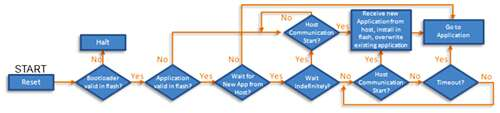
\includegraphics[scale=1]{dados/figuras/FluxoBootloader.jpg}
     \caption{Fluxograma de operações de um bootloader.}
     \label{FluxoBootloader}
\end{figure}



Os sistemas microcontrolados STM32 possuem um \bootloader\ pré programado na ROM desde sua fabricação. Esse \bootloader\ pode utilizar diversos periféricos de comunicação, e para cada periférico diferente a ST padronizou diferentes protocolos que permitem várias operações, como: obter o ID do chip, escrever e ler bytes na RAM e memória flash, apagar setores das memórias, ativar áreas de proteção na memória e pular para o código principal do sistema \cite{Noviello2018}.

É possível ser criado um \bootloader\ customizado com diversas funções adicionais. Uma função frequentemente usada é o uso do \bootloader\ para descriptografar firmwares que podem chegar via internet, para se garantir a segurança e origem do \firmware, assim após esse processo o sistema pode substituir o \software\ anterior pelo recebido. 



\subsection{LINKER}

Segundo \citeonline{Qing2003}, os arquivos de uma aplicação são processados pelo compilador e \textit{assembler}. Criando assim os arquivos objetos, que contém os códigos de máquina binários (\textit{machine binary code}) e dados de programa (\textit{program data}). O \textit{archive utility} concatena uma coleção de arquivos objetos para formar uma biblioteca. Então o \linker\ obtém esses arquivos objetos como entrada e produz ou um arquivo executável, ou um arquivo objeto que pode ser utilizado em outro \linker\ com outros arquivos objetos. O arquivo de comandos de \linker\ (\textit{linker command file}) orienta o \linker\ em como combinar esses diferentes arquivos objetos e aonde colocar o código binário e os dados no sistema embarcado alvo. Assim podemos concluir que, a função principal de um \linker\ é combinar múltiplos arquivos objetos em um arquivo objeto relocável maior, um arquivo objeto compartilhado ou uma imagem executável final. Esse processo pode ser observado na \autoref{linker}.

\begin{figure}[H]
    \scriptsize
     \centering
     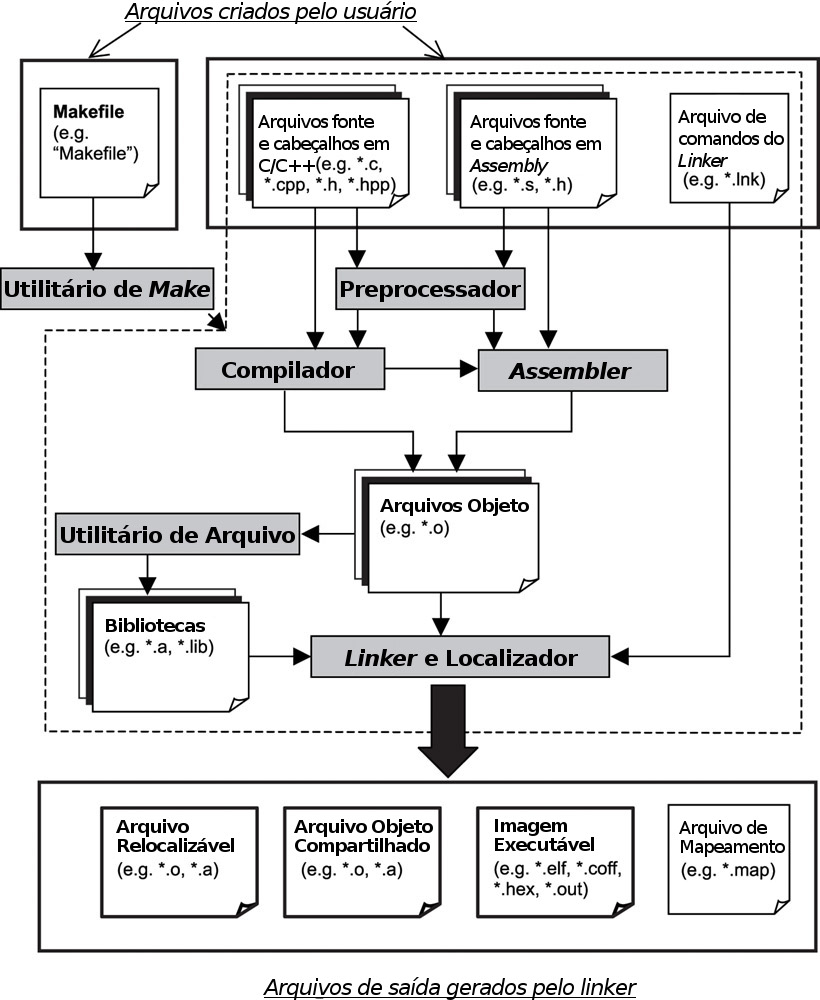
\includegraphics[scale=0.5]{dados/figuras/Linker.png}
     \caption{Criando um arquivo de imagem para um sistema alvo.\newline Fonte:\cite{Qing2003}}
     \label{linker}
\end{figure}

%Durante a compilação de um arquivo fonte, o compilador cria uma tabela de simbolos contendo os simbolos globais e também as referencias para simbolos externos. O processo de \textit{linking}é feito pelo linker envolvendo a resolução de simbolos e relocação de simbolos.
%melhorar esse paragrafo, pagina 22 Qing

%A resolução de simbolos é o processo em que o linker análisa cada arquivo objeto e determina para cada um, em qual outro arquivo ou arquivos objetos, o simbolo esta definido. Quando um simbolo externo esta definido em uma biblioteca estática, o linker copia o arquivo objeto da biblioteca e o escreve na imagem final.

%A relocação de símbolos é o processo em que o linker mapeia a referência desses símbolos para o local de sua definição. O linker modifica o codigo de máquina do arquivo objeto com o intuito de que o código referenciado pelo simbolo reflita o verdadeiro endereço designado a esse símbolo. A tabela de relocação diz ao linker aonde no código do programa aplica a ação de relocação. Cada entrada na tabela de relocação contem a referência para a tabela de símbolos. Utilizando esta referência, o linker pode recuperar o verdadeiro endereço do símbolo e aplicar em determinada parte do programa, como especificado na tabela de relocação. é possivel que a tabela de relocação contenha tanto o endereço do símbolo, quanto a informação da localização em que ele precisa ser realocado. Neste caso, não existe referencia entre as tabelas de relocação e de símbolo.

%A figura \ref{} mostra esses dois processos de forma simplificada.

%\begin{figure}[H]
%    \scriptsize
%     \centering
%     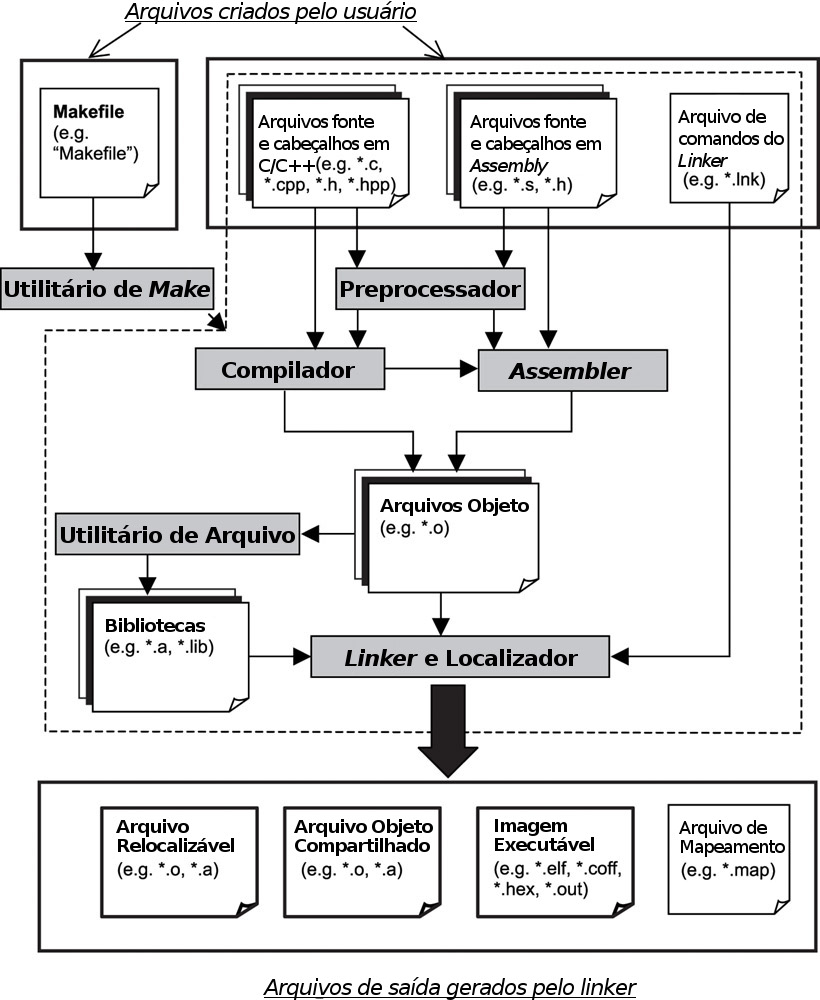
\includegraphics[scale=1]{dados/figuras/Linker.png}
%     \caption{Criando um arquivo de imagem para um sistema operacional alvo.\newline Fonte:\cite{Qing2003}}
%     \label{linker}
%\end{figure}

O \linker\ precisa combinar esses arquivos objetos e fundir as seções de diferentes arquivos em um segmento de programa. Esse processo cria uma única imagem executável para o sistema embarcado alvo. O desenvolvedor utiliza comandos de \linker\ (chamados de \textit{linker directives}) para controlar como o \linker\ combina essas seções e aloca seus segmentos no sistema alvo. As diretivas de \linker\ ficam contidas no arquivo de comando de \linker. O objetivo de criar esse arquivo de comando de \linker\ é para que o desenvolvedor de sistemas embarcados possa mapear a imagem executável para o \textit{hardware} alvo de forma precisa e eficiente. 

\begin{figure}[H]
    \scriptsize
     \centering
     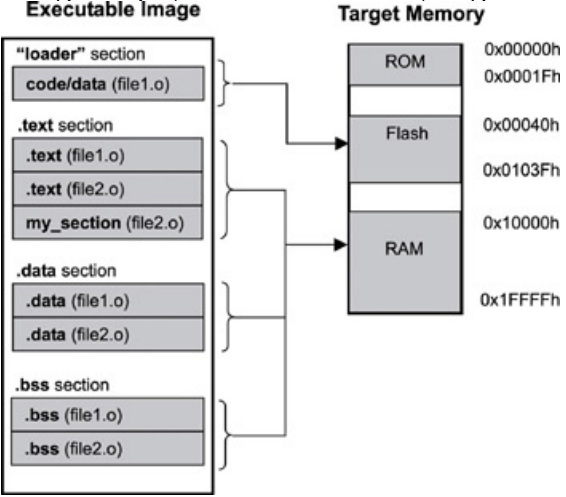
\includegraphics[scale=0.7]{dados/figuras/Linker4.png}
     \caption{Mapeando uma imagem executável em um sistema alvo.\newline Fonte:\cite{Qing2003}}
     \label{linker}
\end{figure}







\section {COMUNICAÇÃO CLIENTE-SERVIDOR}

Um programa cliente é um programa que funciona em um sistema computacional, que solicita e recebe um serviço de um programa servidor, que funciona em outro sistema final. Uma vez que o programa cliente é executado em um computador e o programa servidor, é executado em outro, aplicações cliente-servidor são, por definição, aplicações distribuídas. Os programas cliente e o servidor interagem enviando mensagens um para o outro, pela internet ou qualquer outra rede local ou remota. Neste nível de abstração, os roteadores, enlaces e outros componentes da internet funcionam como uma caixa-preta que transferem mensagens entre os componentes distribuídos, comunicantes, de uma aplicação \cite{Kurose2010}.

A comunicação cliente-servidor na internet é feita por meio de diversos protocolos de rede, cujo conjunto de protocolos é conhecido como pilha TCP/IP (\textit{Transmission Control Protocol/Internet Protocol}). Essa pilha é dividida em quatro camadas, em que cada camada é encarregada de realizar uma série de funções, concedendo um grupo de serviços bem definidos para o protocolo da camada superior. A \autoref{fig:PilhaTCP} ilustra a pilha TPC/IP e seus protocolos. 

\begin{figure}[H]
    \scriptsize
     \centering
     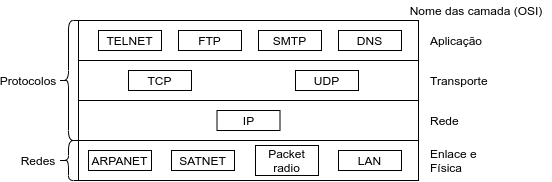
\includegraphics[scale=1]{dados/figuras/PilhaTCP-IP.png}
     \caption{Pilha TCP/IP e seus protocolos.\newline Fonte:\cite{tanenbaumRedes}}
     \label{fig:PilhaTCP}
\end{figure}

Essas camadas são denominadas:

\begin{itemize}
    \item Camada de aplicação: em que residem os protocolos de nível mais alto. Um protocolo da camada de aplicação é distribuído por diversos sistemas finais, sendo que a aplicação em um sistema usa o protocolo para trocar pacotes de informação com a aplicação em outro sistema.
    Exemplos de protocolos:
    \begin{itemize}
        \item HTTP (\textit{Hypertext transfer protocol}).
        \item SMTP (\textit{Simple Mail Transfer Protocol}). 
        \item FTP (\textit{File Transfer protocol}).
        \item DNS (\textit{Domain Name System}).
    \end{itemize}
    \item Camada transporte: em que reside os protocolos que fazem o transporte de dados da camada de aplicação, transportando mensagens entre os lados do cliente e do servidor de uma aplicação.
    Exemplos de protocolos:
    \begin{itemize}
        \item TCP (\textit{Transmission Control Protocol}).
        \item UDP (\textit{User Datagram Protocol}).
    \end{itemize}
    \item Camada de rede: camada que contém o protocolo responsável pela movimentação, de uma máquina para outra, de pacotes de camada de rede conhecidos como datagramas. Um protocolo da camada de transporte passa um segmento TCP ou UDP e um endereço de destino à camada de rede. A camada de rede prove o serviço de entrega do segmento à camada de transporte da máquina destinatária. O protocolo da camada de rede é chamado de IP (\textit{Internet Protocol}).
    \item Camada de enlace: é a camada que contém os protocolos que ficam responsáveis por enviar datagramas de um nó a outro, ou seja, faz o transporte do datagrama entre elementos da rede, como de uma máquina ao roteador, ou de roteador para roteador. Exemplos de protocolos:
    \begin{itemize}
        \item Arpanet.
        \item LAN (\textit{local area network}).
        \item WLAN (\textit{wireless local area network}).\newline
    \end{itemize}

\end{itemize}

Com a popularização da internet essa comunicação se tornou cada vez mais comum, atingindo bilhões de usuários no mundo todo. Assim a comunicação cliente servidor precisa ser segura. A segurança de redes se preocupa em garantir que pessoas mal-intencionadas não leiam ou modifiquem secretamente mensagens enviadas a outro destinatário. Ela também lida com meio de identificar se uma mensagem recebida é verdadeira e tem uma origem confiável \cite{tanenbaumRedes}.



\subsection{LWIP}
%Com a necessidade de se obter os binários dos códigos do novo firmware o sistema irá se utilizar da biblioteca amplamente conhecida e utilizada LWIP.
A Biblioteca LwIP é uma implementação da pilha TCP/IP, focada em ser pequena e portável, reduzindo a utilização de recursos como memória RAM e ainda tendo um TCP completo, se tornando adequada para sistemas embarcados. Foi originalmente desenvolvida por Adam Dunkels nos laboratórios da \textit{Computer and Networks Architectures} (CNA), no Instituto Sueco de Ciência da Computação (SICS) e agora é desenvolvida e mantida por uma rede mundial de desenvolvedores \cite{LWIP}.

Possui três \textit{Aplication Programing Interfaces} (APIs):
\begin{itemize}
\item RAW API (API básica): É a API nativa do LwIP, possui melhor desempenho e o menor tamanho de código, porém torna o desenvolvimento de aplicações mais complexo.
\item Netconn API: É uma API sequencial de alto nível que requer um sistema operacional de tempo real (RTOS). Habilita operações com múltiplas \textit{threads}.
\item BSD Sockets API: API de \textit{sockets} de Berkeley, desenvolvida em cima da API Netconn.
\end{itemize}

Essas API's implementam diversos protocolos de rede, incluindo:
\begin{itemize}
    \item HTTP permite a obtenção de recursos, tais como documentos HTML, imagens, scripts e outros tipos de arquivos.
    \item FTP para o envio e recebimento de arquivos.
    \item SMTP para o envio de mensagens de correio eletrônico através da internet.
    \item ICMP (\textit{Internet Control Message Protocol}) para manutenção e \textit{debugging} da rede.
    \item TCP com controle de congestionamento, estimativa de latência, recuperação e retransmissão rápida.
    \item IP incluindo o envio de pacotes para múltiplas interfaces de rede. \newline
    
 
    
\end{itemize} 

A seguir serão explanados com mais profundidade alguns dos protocolos implementados pela LwIP que serão utilizados neste trabalho.

\subsubsection{HYPERTEXT TRANSFER PROTOCOL (HTTP)}
Segundo \citeonline{Kurose2010}, o protocolo da camada de aplicação HTTP é implementado em dois programas, um programa cliente e outro servidor. Os dois são executados em sistemas finais diferentes, se comunicam entre eles por meio de uma troca de mensagens HTTP. O HTTP define a estrutura dessas mensagens assim como o modo como o cliente e o servidor as trocam. 

O HTTP define como clientes requisitam documentos aos servidores e como eles os transferem ao cliente. Ele utiliza o TCP como seu protocolo de transporte subjacente. O cliente HTTP primeiramente inicia uma conexão TCP com o servidor. Após essa conexão ser estabelecida, os processos da aplicação e do servidor acessam o TCP por meio de sua interface de sockets. No lado do cliente a interface de socket é uma porta entre o processo cliente e a conexão TCP. No lado do servidor, ela é uma porta entre o processo servidor  e a conexão TCP.

O cliente envia mensagens de requisição HTTP para sua interface de socket e recebe uma mensagem de resposta HTTP de sua interface de socket. De uma maneira parecida acontece do lado do servidor, onde ele recebe mensagens de requisição HTTP de sua interface de socket e envia mensagens respostas a sua interface. Assim a mensagem sai da camada de aplicação e passa para a camada de transporte. 

\subsubsection{TRANSMISSION CONTROL PROTOCOL (TCP)}

Segundo \citeonline{tanenbaumRedes}, O TCP foi projetado especificamente para oferecer um fluxo de bytes fim a fim confiável em uma inter-rede não-confiável. Uma inter-rede é diferente de uma única rede porque suas diversas partes podem ter topologias, larguras de banda, retardos, tamanhos de pacotes e outros parâmetros totalmente diferentes. O TCP foi projetado para se adaptar dinamicamente às propriedades da inter-rede e ser robusto diante de muitos categorias de falhas que podem ocorrer.

Cada máquina compatível com TCP tem uma entidade de transporte TCP, que pode ser um procedimento de biblioteca, um processo do usuário ou parte do núcleo. Em todos os casos, ele gerencia fluxos e interfaces TCP para a camada IP. Uma entidade TCP aceita fluxos de dados de usuários provenientes de processos locais, divide-os em partes de no máximo 64 kB e envia cada parte em um datagrama IP distinto. Quando os datagramas IP que contem dados TCP chegam a uma máquina, eles são enviados à entidade TCP, que restaura o fluxo de bytes originais.

A camada IP não oferece garantia que os datagramas serão entregues de forma apropriada, portanto, cabe ao TCP administrar os \textit{timers} e retransmiti-los sempre que necessário. Os datagramas também podem chegar fora de ordem, o TCP também terá que os reorganizar em mensagens na sequência correta. 

\subsection{MBED TLS}
A biblioteca Mbed TLS foi desenvolvida para se integrar facilmente a aplicações embarcadas existentes, e fornecer os blocos de construção para uma comunicação segura, criptografia e gerenciamento de chaves. Como o seu intuito é ser o mais flexível possível, permite que sejam integrados ao sistema somente as funcionalidades necessárias, diminuindo assim o tamanho total que a biblioteca ocuparia no sistema \cite{mbedtls}.

A \autoref{mbedtlsFig} ilustra como a biblioteca cria uma camada intermediária entre a aplicação final e a camada TCP/IP, chamada de TLS (\textit{Transport Layer Security}). A Mbed TLS pode ser usada para criar um servidor e cliente SSL (\textit{Secure Sockets Layer})/TLS, fornecendo uma estrutura para a configurar e se comunicar por meio de um canal de comunicação SSL/TLS. A camada TLS criada depende diretamente dos módulos de análise de certificado, criptografia simétrica ou assimétrica e \hash\ da biblioteca utilizada.

\begin{figure}[H]
    \scriptsize
     \centering
     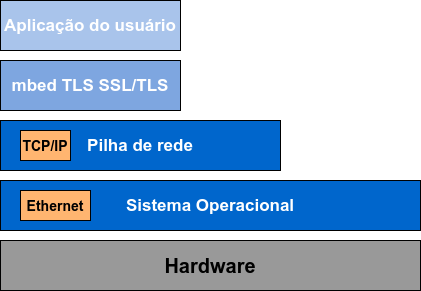
\includegraphics[scale=1]{dados/figuras/mbedtls.png}
     \caption{Pilha de comunicação.\newline Fonte:\cite{mbedtls}}
     \label{mbedtlsFig}
\end{figure}

A Mbed TLS provê a implementação da camada de segurança para a comunicação com o servidor, que pode evitar que uma versão maliciosa do software seja recebida de uma fonte não confiável. Também nos fornece peças de software contendo algoritmos criptográficos, que podem ser facilmente acoplados a qualquer aplicação. Como é o caso do algoritmo SHA-2 que ficará responsável por fazer a verificação da integridade dos arquivos baixados.

\subsubsection{TRANSPORT LAYER SECURITY (TLS)}

A \textit{Transport Layer Security} assim como seu precursor \textit{Secure Sockets Layer}, é um protocolo de segurança projetado para fornecer segurança na comunicação sobre uma rede de computadores.
Segundo \citeonline{TLSV12}, o protocolo TLS visa fornecer privacidade e integridade de dados entre aplicações que se comunicam. Quando uma rede está protegida por TLS, conexões entre um cliente e um servidor devem ter uma ou mais das seguintes propriedades:

\begin{itemize}
    \item A conexão é privada, pois, utilizada criptografia simétrica para criptografar os dados transmitidos. As chaves para essa criptografia são geradas exclusivamente para cada conexão e são baseadas em um segredo compartilhado que foi negociado no início da sessão (conhecido como \textit{Handshake Protocol}). No protocolo de \textit{Handshake}, o servidor e o cliente negociam qual algoritmo de criptografia e chaves criptográficas usar antes que o primeiro dado seja transmitido. Como a negociação ocorre somente no início da transmissão, qualquer invasor que intercepte a transmissão não poderá decifrar as mensagens, enviar dados e alterar os termos dessa negociação. Então a negociação de um segredo compartilhado é segura  e confiável.
    \item A conexão é confiável, pois cada mensagem transmitida inclui uma verificação de integridade de mensagem, utilizando um código de autenticação de mensagem, como uma \textit{hash} criptográfica, para evitar perda não detectada ou alteração dos dados durante a transmissão.
\end{itemize}

Uma vantagem do TLS é que ele é independente do protocolo da aplicação. No entanto, ele não especifica como os protocolos adicionam segurança ao TLS, as decisões sobre como iniciar o \textit{handshaking} e como interpretar os certificados de autenticação trocados são deixadas ao critério dos projetistas e desenvolvedores de protocolos executados sobre o TLS.

\subsubsection{FUNÇÃO HASH}

Segundo \citeonline{Kurose2010}, uma função \textit{hash} é um algoritmo que recebe uma entrada, $m$, e computa uma cadeia de bits de tamanho fixo $H(m)$ conhecida como \textit{hash}. Uma função de \textit{hash} criptográfica deve apresentar a seguinte propriedade:
no processamento, é impraticável encontrar duas mensagens diferentes $x$ e $y$ em que $H(x)=H(y)$.

A SHA-1 (Secure \textit{Hash} Algorithm) é um conjunto de funções \textit{hash} criptográficas projetadas pela NSA\cite{NSA}. Esse algoritmo, de forma resumida, se baseia em processar um resumo de mensagem de 160 bits por meio de um processo de quatro etapas, formado por uma etapa de enchimento(Adicionando 'uns' seguidos de 'zeros' suficientes, de maneira em que o comprimento da mensagem satisfaça determinados critérios), uma etapa de anexação (anexação de uma representação de alguns bits do comprimento da mensagem antes do enchimento), uma etapa de inicialização de um acumulador e uma etapa final iterativa, em que os blocos de palavras da mensagem são processados (misturados) em quatro rodadas de processamento. 

Comparando o \hash\ computado (a saída de execução do algoritmo) a um valor de \hash\ conhecido e esperado, pode-se determinar a integridade dos dados. Por exemplo, calcular o \hash\ de um arquivo baixado e comparar o resultado com um \hash\ conhecido, pode comprovar que o arquivo foi modificado ou adulterado.
SHA-2 é um conjunto de funções \hash\ criptográficas que contém mudanças significativas de seu antecessor. É composta por seis funções \hash\ com valores de \hash\ que são de 224, 256, 384 ou 512 bits: SHA-224, SHA-256, SHA-384, SHA-512, SHA-512/224, SHA-512/256.



%\section{CARTÃO SD}
\section{SISTEMAS DE ARQUIVO}
Segundo \citeonline{tanenbaumSO}, para resolver diversos problemas com o armazenamento de grandes quantidades de dados, a perda de dados após o fim da execução do processo que os criou e a necessidade de tornar esses dados independentes de quaisquer processos. Existe a necessidade da criação de uma estrutura de armazenamento de informações a longo prazo. Os três requisitos fundamentais para essa estrutura são:

\begin{itemize}
    \item Deve ser possivel armazenar um volume grande de informações.
    \item Os dados devem sobreviver ao término do processo que os estão utilizando.
    \item Vários processos devem ser capazes de acessar os dados concomitantemente.
\end{itemize}

Essa estrutura é chamada de arquivo, e é vastamente utilizada por diversos sistemas. Os arquivos são utilizados para armazenar dados em discos e outras mídias externas. Então os processos podem ler e escrever novos dados quando necessário. As informações armazenadas em arquivos devem ser persistentes, logo, não devem ser afetadas pela criação e pelo término do processo. Um arquivo só deve desaparecer quando o seu criador o apagar.

O modo como os arquivos são estruturados, nomeados, acessados, usados, protegidos e implementados são definidos geralmente pelo sistema operacional. A parte do sistema operacional responsável por esse gerenciamento é chamada de sistema de arquivos. Os arquivos podem, no caso de sistemas embarcados, ser gerenciados por API's que criam uma camada independente do sistema operacional e gerenciam os arquivos, como é o caso da biblioteca FatFs. 

Existem diversas formas de implementar um sistema de arquivo. Nessa implementação é necessário saber como os arquivos e seus diretórios são armazenados, como o espaço em disco é gerenciado e em como fazer tudo funcionar de modo eficiente e confiável. 
Um dos sistemas de arquivos padrões para o uso em memórias que são divididas em bloco é o FAT32. 
Um cartão SD é um dispositivo de memória não volátil criado pela SD Card Association \cite{SDCARD}, que possui sua memória dividida em blocos e que por padrão faz uso do sistema de arquivo FAT.




\subsection{SISTEMA DE ARQUIVO FAT}

Segundo \citeonline{tanenbaumSO}, o sistema de arquivo FAT (\textit{File Allocation Table}) é implementado por meio de uma alocação de memória encadeada usando uma tabela na memória. Nessa organização, o bloco de memória inteiro está disponível para dados. Além disso, o acesso aleatório é muito mais fácil. Mesmo que o encadeamento ainda tenha que ser seguido para encontrar determinado deslocamento dentro do arquivo, ele está inteiramente na memória. De modo que, pode ser seguido sem necessidade nenhuma de referenciar o disco.

A \autoref{FAT} ilustra como é a tabela, mostrando que o arquivo $A$ inicia-se no bloco 4 e segue o encadeamento até o seu fim, assim como o arquivo $B$ que se inicia no bloco 6. Ambos terminam com um marcador especial que no caso é o número -1.

\begin{figure}[H]
    \scriptsize
     \centering
     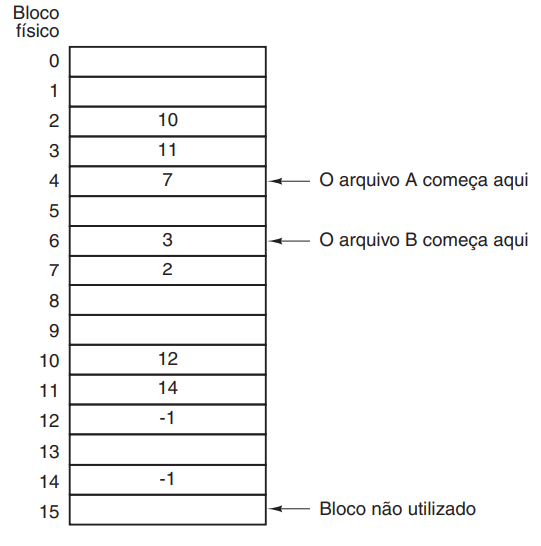
\includegraphics[scale=0.7]{dados/figuras/FAT.png}
     \caption{Alocação encadeada usando tabela de alocação de arquivo.\newline  Fonte:\cite{tanenbaumSO}}
     \label{FAT}
\end{figure}

A principal desvantagem deste método é que a tabela inteira precisa estar na memória o tempo todo. Com um disco de 20 GB e um tamanho de bloco de 1 KB, a tabela precisa de 20 milhões de entradas, uma para cada um dos 20 milhões de blocos do disco. Cada entrada tem de ter no mínimo 3 bytes para manter o endereço dos blocos. Para facilitar sua pesquisa, as entradas acabam ocupando 4 bytes. Assim, a tabela ocupará 60 MB ou 80 MB de memória principal o tempo todo, dependendo do sistema para ser otimizado para espaço ou para tempo.

Existe também o sistema de arquivo exFAT que é utilizado para mídias com capacidade de armazenamento maiores que 4 GB, que foi adotada como sistema de arquivo padrão para cartões de memória (SD card) maiores de 4 GB, pela SD Card Association \cite{SDCARD}.

\subsection{FATFS}

FatFs é um módulo genérico de um sistema de arquivo FAT/exFAT, para pequenos sistemas embarcados com recursos computacionais reduzidos. É escrito em conformidade com a ANSI C (C89) e é completamente separado da camada de entrada e saída do sistema, portanto, é independente da plataforma utilizada. É um \software\ livre de código aberto e proporciona a leitura, escrita, criação e remoção de arquivos, além do gerenciamento e navegação de diretórios. A \autoref{FatFS} ilustra como o módulo é independente da aplicação e da plataforma utilizada.

\begin{figure}[H]
    \scriptsize
     \centering
     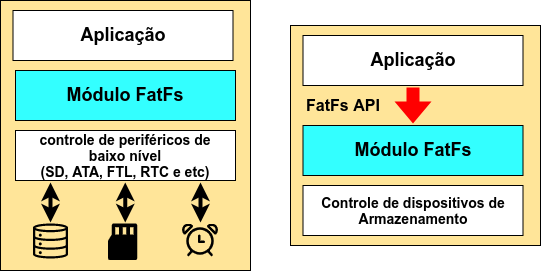
\includegraphics[scale=0.6]{dados/figuras/fatfs.png}
     \caption{Posição da biblioteca FatFs na aplicação.\newline  Fonte:\cite{FATFS}}
     \label{FatFS}
\end{figure}
A FatFs fornece várias funções do sistema de arquivos para a aplicação.
Assim pela aplicação é possível gerenciar os arquivos e diretórios, como é ilustrado da \autoref{FatFS2}. Umas das principais funções fornecidas pela FatFs para a aplicação são:

\begin{itemize}
    \item Acesso a arquivos.
    \begin{itemize}
        \item f\_open - Abre/Cria um arquivo.
        \item f\_close - Fecha um arquivo aberto.
        \item f\_read - Lê os dados de um arquivo.
        \item f\_write - Escreve dados em um arquivo.
    \end{itemize}
    \item Acesso a diretórios.
    \begin{itemize}
        \item f\_opendir - Abre um diretório.
        \item f\_closedir - Fecha um diretório aberto.
    \end{itemize}
    \item Gerenciamento de arquivos e diretórios.
    \begin{itemize}
        \item f\_stat - Verifica a existência de um arquivo ou diretório.
        \item f\_unlink - Remove um arquivo ou diretório. 
        \item f\_rename - Renomeia ou move um arquivo, ou diretório.
        \item f\_mkdir - Cria um diretório.
        \item f\_chdir - Muda o diretório atual.
    \end{itemize}
    \item Gerenciamento de volume e configurações do sistema.
    \begin{itemize}
        \item f\_mount - Registra ou remove registro da área de trabalho da partição.
        \item f\_mkfs - Cria uma partição FAT na unidade lógica.
        \item f\_fdisk - Cria uma partição na unidade física.
        \item f\_getfree - Obtém o espaço livre da partição.
    \end{itemize}
\end{itemize}

\begin{figure}[H]
    \scriptsize
     \centering
     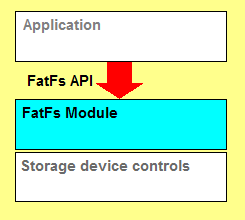
\includegraphics[scale=0.6]{dados/figuras/fatfs2.png}
     \caption{Manipulação da memória por meio da API da FatFs.\newline  Fonte:\cite{FATFS}}
     \label{FatFS2}
\end{figure}
%\section{SERVIDORES HTTP}

%É uma boa prática iniciar cada novo capítulo com um breve texto introdutório (tipicamente, dois ou três parágrafos) que deve deixar claro o quê será discutido no capítulo, bem como a organização do capítulo.
%Também servirá ao propósito de "amarrar"{} o conteúdo deste capítulo com o conteúdo do capítulo imediatamente anterior.


\section{TRABALHOS CORRELATOS}

Foram identificados três trabalhos correlatos.

%pode ter latencia de interrupção porem deve ser controlada

\begin{itemize}

    \item \textbf{Firmware over the air for automotive, Fotamotive}: Esse trabalho introduz uma solução para atualização de veículos com a ajuda de fabricantes de equipamentos altomotivos para reduzir custos com \textit{recalls} e assim aumentar a qualidade de seus produtos, facilitar as atualizações e controlar melhor a frota de veículos no mercado. Essa solução consiste em atualizar a unidade de controle do motor por meio de métodos OTA, sem a necessidade de uma conexão física com o veículo \cite{Odat2014}.

    \item \textbf{Firmware over the air for home cybersecurity in the Internet of Things}: Esse trabalho descreve a utilização de um método de atualização de \firmware\ para roteadores caseiros, utilizando sistemas de gerenciamento de rede e de suporte de operações de fornecedores de acesso à \textit{internet} \cite{Teng2017}.
    
    \item \textbf{Internet of Things: Over-the-Air (OTA) firmware update in Lightweight mesh network protocol for smart urban development}: Esse trabalho introduz um novo sistema de atualização de \firmware\ \textit{Over-The-Air} (OTA) baseado no protocolo de rede \textit{Lightweight mesh}, que prove descoberta de rotas, estabelecimento e um protocolo de malha de baixa potência \cite{Chandra2016}.

\end{itemize}

Como observado, todos os trabalhos correlatos tem um objetivo único e diferente para a aplicação de sua atualização OTA, enquanto esse trabalho tem como meta produzir um sistema que pode abranger diferentes aplicações.